%! Author = Saeid Yazdani
%! Date = 8/10/2024


\section{Control loop details}
\label{sec:loopdetails}

\autoref{fig:loop-algo} shows the high-level block diagram of the control loop
components.

The control loop algorithm starts from data that are generated from analog
signals by the \ac{ADC} modules.
Data correction for \emph{offset} and full-scale range gain settings precedes
range scaling to the control loop's SET DAC.

The \acs{FPGA} manages \emph{Compensation}, \emph{\acs{DAC}} and
\emph{\acs{ADC}} blocks and controls all the dynamic operations:

\begin{itemize}[topsep=8pt,itemsep=4pt,partopsep=4pt, parsep=4pt]
    \item Repetitive reading of all ADC values coming from five ADC chips
    through the \ac{LVDS} interface.

    \item Calculation of control loop signals sent to the control loop DAC for:
    \begin{itemize}[topsep=8pt,itemsep=4pt,partopsep=4pt, parsep=4pt]
        \item Offset correction,
        \item \acs{FSR} Scaling, over-range limitation (clamp function),
        \item Data correction and re-scaling for the DAC \acs{FSR}
    \end{itemize}

    \item Transfer and receive runtime data to and from the registers to
    \ac{MCU} using the parallel bus.
    \item Output of the compensation data (dynamic loop control) as pre-defined
    by the \ac{MCU}.

\end{itemize}

In any control loop, we compensate the control amplifier's \emph{SET} input
signal such that the output signal reaches the \emph{target} value.
We get a \emph{zero} input signal only if the amplifier’s gain is infinity – in
a practical approach we use an input signal of $V_{OUT}$ and \emph {GAIN} at the
summing point – the lower the gain the higher the summing node signal.

Output current is measured using shunt resistors for given output ranges
in a high-side current measurement configuration.
The current sense signal is transferred to the control system via optically
isolated data communication lines.

If the control input is switched to the \emph{Current Sense} signal we get a
current source and the voltage \emph{clamp} is activated.

\begin{figure}[htbp]
    \centering
    \printfitgraphics[0.62\textheight]{figures/design-realization/hvs-control-overview}
    \caption[\acs{FPGA} Control Loop Diagram]{
        High-level block diagram of the control loop components inside
        the FPGA.
    }
    \label{fig:loop-algo}
\end{figure}

\subsection{Input Processing}
\label{subsec:input-processing}

\autoref{fig:fpga-input-block_fpga_input_processing} shows the flow of
data for processing control loop output value inside the FPGA.
An optional moving average window and an inverter stage are provisioned.
Data acceptance can be paused to inject test data to debug the control loop.

\begin{figure}[h]
    \centering
    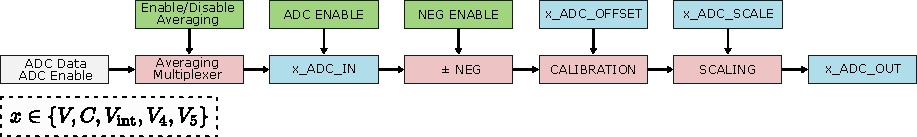
\includegraphics[width=1\textwidth]
    {figures/design-realization/fpga_input_processing}
    \caption[FPGA Input processing]{
        Overview of data flow for processing loop variables by the FPGA.
    }
    \label{fig:fpga-input-block_fpga_input_processing}
\end{figure}

There are five ADC blocks with 4 dedicated registers assigned to each.
These registers (5x4) associated with \ac{ADC} chips are mapped to address
ranges \texttt{0x00} to \texttt{0x13}.
The input blocks are performing the following tasks during runtime:

\begin{itemize}[topsep=8pt,itemsep=4pt,partopsep=4pt, parsep=4pt]
    \item{Continuous reading of all ADC values (five ADC)}
    \item{Calculation of appropriate control loop settings}
    \item {Continuous output of DAC values}
\end{itemize}

All measured values from the ADC are corrected in the first step according
to individual correction data, scaled to the target range of the DAC, and
then transferred to the DAC for proper control loop operation.
All ADC values are stored in a \ac{DPRAM} buffer on the FPGA for further
analysis.

A moving average window is available, data acceptance can be stopped for
injecting test data, and an inverter stage is available.

\subsection{Output Processing}
\label{subsec:output-processing}


The input data for the loop's set DAC are combined data from \emph{SET} and
\emph{VERNIER} (alternatively used for \emph{offset}) and \emph{COARSE}.
All data are scaled (\texttt{1.0} = \texttt{0x1000}) and offset (signed integer) to
adjust the number representations.
The 12 DAC registers (3x4) are mapped to address \texttt{0x14} to
\texttt{0x1F}.

\subsection{Calibration of \acs{DAC} and \acs{ADC}}
\label{subsec:dac-and-adc-calibration}

The physical components of the system especially in the \acs{ADC} and \acs{DAC}
blocks can drift as a result of aging and environmental effects such as
temperature and humidity.
Therefore, range adjustments and offset corrections are necessary to compensate for
these variations to ensure the system maintains accuracy and reliability.
Range adjustment is necessary to prevent the output from exceeding the
operational limits of the components of the system.
\autoref{table:fsr-range-adjustments} shows the provisioned values for range
adjustment.

\begin{table}[h]
    \centering
    \begin{tabular}{c|c|c}
%        \hline
        \multicolumn{3}{c}{\small \textbf{Range Adjustment for \acs{DAC} and \acs{ADC}}} \\ \cline{1-3}
        \texttt{0x7FFF} & maximum value     & \texttt{0xFFFF} \\ \hline
        \texttt{0x0000} & zero              & \texttt{0x8000} \\ \hline
        \texttt{0x8000} & - (maximum value) & \texttt{0x0000} \\ \hline
    \end{tabular}
    \caption[\acs{DAC} and \acs{ADC} Range Adjustments]{
        Range adjustments for all DAC and ADC modules ensure that the input and
        output signals are appropriately scaled to match their \acs{FSR}.
    }
    \label{table:fsr-range-adjustments}
\end{table}

The DAC and ADC drifts are corrected via dedicated offset \emph{offset}
registers.
For example, an analog \SI{0}{\volt} should be generated for a
\acs{DAC} value of \texttt{0x0000}.
But instead, we may get \SI{4}{\milli\volt} of deviation.
This deviation will be the calibration value equal to
\texttt{0xFFF1} (\SI{-4}{\milli\volt}) for this particular DAC value.
The output is then corrected to \SI{0}{\volt}.
ADC modules in the system also may show a slight offset resulting in small
non-zero values such as \texttt{0x0008} to be generated for a \SI{0}{\volt}
input, hence it is also necessary to calibrate and correct the ADC values.

The calibration procedure can be done for every bit of the \acs{FSR} or with a
skip factor and normalization over the skipped range with a tradeoff
between precision and execution time.
Dedicated calibration blocks in the \acs{FPGA}
are tasked to correct DAC and ADC values using the offset factors
saved in calibration \ac{LUT} as shown in \autoref{fig:dac-adc-calib}.

\begin{figure}[h]
    \centering
    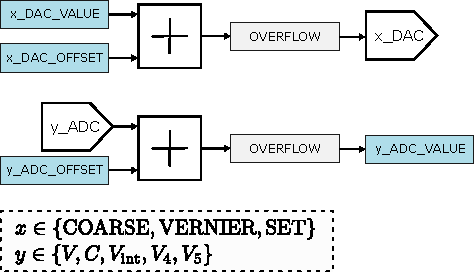
\includegraphics[width=0.7\textwidth]
    {figures/design-realization/adc-and-dac-calibration}
    \caption[Calibration of ADC and DAC]{
        Calibration blocks for \acs{DAC} (top) and \acs{ADC} (bottom).
    }
    \label{fig:dac-adc-calib}
\end{figure}

\subsection{Scaling \acs{ADC} and \acs{DAC} values}
\label{subsec:scaling-adc-dac}

At different voltage and current ranges, the adjusted range from ADC to DAC
blocks may not align correctly due to:

\begin{itemize}[topsep=8pt,itemsep=4pt,partopsep=4pt, parsep=4pt]
    \item \textbf{Range Mismatch:}
    The ADC might be converting the input signal to a digital value over a
    different range than the DAC expects.

    \item \textbf{Gain Differences:}
    If the gain applied by the ADC is different from that expected by the DAC,
    the digital data might not represent the analog signal accurately when
    converted back by the DAC.

\end{itemize}

In such cases, scaling is a necessary step if the measured and offset-corrected
ADC data does not match the output of the DAC.
The scaling operation is done by multiplying ADC values by a dedicated block
inside the FPGA as shown in \autoref{fig:dac-adc-scaling}.

\begin{figure}[h]
    \centering
    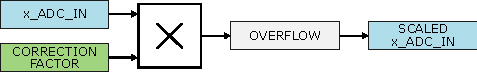
\includegraphics[width=0.7\textwidth]
    {figures/design-realization/fpga-adc-dac-scaling}
    \caption[ADC-DAC Scaling]{
        Block diagram of the scaling operation inside the FPGA.
    }
    \label{fig:dac-adc-scaling}
\end{figure}

The scale factor is generated through reference data collection and maintenance
procedures that involve supplying test signals into ADC chips and recording
their outputs.
These ADC outputs will be sent to corresponding DACs and the resulting analog
outputs will be recorded.
The scale factor for a given bit or range of bits is then calculated
according to \autoref{eq:scale-factor}.

\begin{equation}
    \label{eq:scale-factor}
    \text{Scale Factor} = \frac{\text{Expected Output}}{\text{Actual Output}}
\end{equation}

When the voltage ADC or the current ADC reaches their \acs{FSR} limits, we need
to lower the set point voltage until the ADC readings return to non-limited
values.
Therefore, a \emph{re-scaling} or \emph{scale-limiting} block is necessary to
prevent clipping.

\begin{figure}[h]
    \centering
    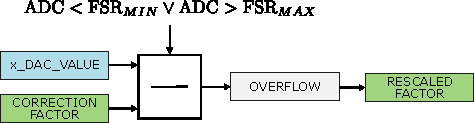
\includegraphics[width=0.7\textwidth]
    {figures/design-realization/adc-rescaling}
    \caption[Scale Limiter]{
        Block diagram of scale-limiter inside the \ac{FPGA}.
    }
    \label{fig:scale-limiter}
\end{figure}

\subsection{\acs{ADC} Averaging}
\label{subsec:adc-averaging}

ADC readings can be affected by random electrical noise, which causes small
fluctuations in the output.
Averaging multiple samples helps smooth out these fluctuations and yield
accurate and stable representation of the signal.

As stated before, an optional averaging block is provisioned in the \ac{FPGA}
with configurable window sizes of 2, 4, 8, and 16 samples that can be enabled or
bypassed for faster response, as averaging will result in slower response time
and reduced temporal resolution, affecting the dynamic behavior of the system
especially in transient events.

The averaging operation is done in the FPGA by division operation over
the sum of selected data samples according to the window size as shown in
\autoref{fig:adc-averaging}.

\begin{figure}[h]
    \centering
    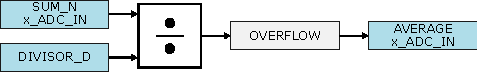
\includegraphics[width=0.7\textwidth]
    {figures/design-realization/fpga_averaging}
    \caption[ADC Value Averaging]{
        Block diagram of the averaging operation inside the FPGA.
    }
    \label{fig:adc-averaging}
\end{figure}

\subsection{RAM Analysis}
\label{subsec:ram-analysis}

The system stores $2^{16}$ ADC samples every time that a new SET DAC value has
been applied.
We can skip a pre-defined number of samples for storing using ACCESS\_CNT
registers individually per Voltage ADC and Current ADC dedicated registers.
This allows for the acquisition of different waveforms in current and voltage.
The microcontroller can read these data for further processing.

